\documentclass[border=10pt]{standalone}
\usepackage{tikz}
\usetikzlibrary{positioning, arrows.meta}
\usepackage{xcolor}
\usepackage[T1]{fontenc}
\usepackage{lmodern}

%% ── Palette ──────────────────────────────────────────────────────────────────
\colorlet{cN}{black!52}
\colorlet{cL}{orange!85!red}
\colorlet{cP}{violet!80}
\colorlet{cG}{blue!72!black}
\colorlet{cWin}{green!45!black}
\colorlet{cLoss}{red!62!black}

\tikzset{
  %% Column header
  MH/.style={draw=#1!80!black, fill=#1, text=white, rounded corners=3pt,
             text width=3.5cm, minimum height=0.62cm,
             align=center, font=\small\bfseries},
  %% Retrieval description box
  RB/.style={draw=gray!38, fill=white, rounded corners=2pt,
             text width=3.3cm, minimum height=2.85cm,
             inner sep=5pt, align=left, font=\scriptsize},
  %% Prompt label on arrow
  PL/.style={font=\tiny\itshape, text=gray!65, midway, right=1pt},
  %% Answer box
  AB/.style={draw=#1!55, fill=#1!7, rounded corners=2pt,
             text width=3.3cm, minimum height=2.7cm,
             inner sep=5pt, align=left, font=\scriptsize},
  %% Judge header bar
  JBar/.style={draw=gray!48, fill=gray!10, rounded corners=3pt,
               text width=14.6cm, minimum height=0.62cm,
               align=center, font=\small\bfseries, text=black!65},
  %% Win / Loss circle
  Vc/.style={circle, minimum size=0.52cm, inner sep=0pt,
             font=\bfseries\tiny, text=white},
  %% Generic arrow
  Arr/.style={->, semithick, gray!62},
}

\begin{document}
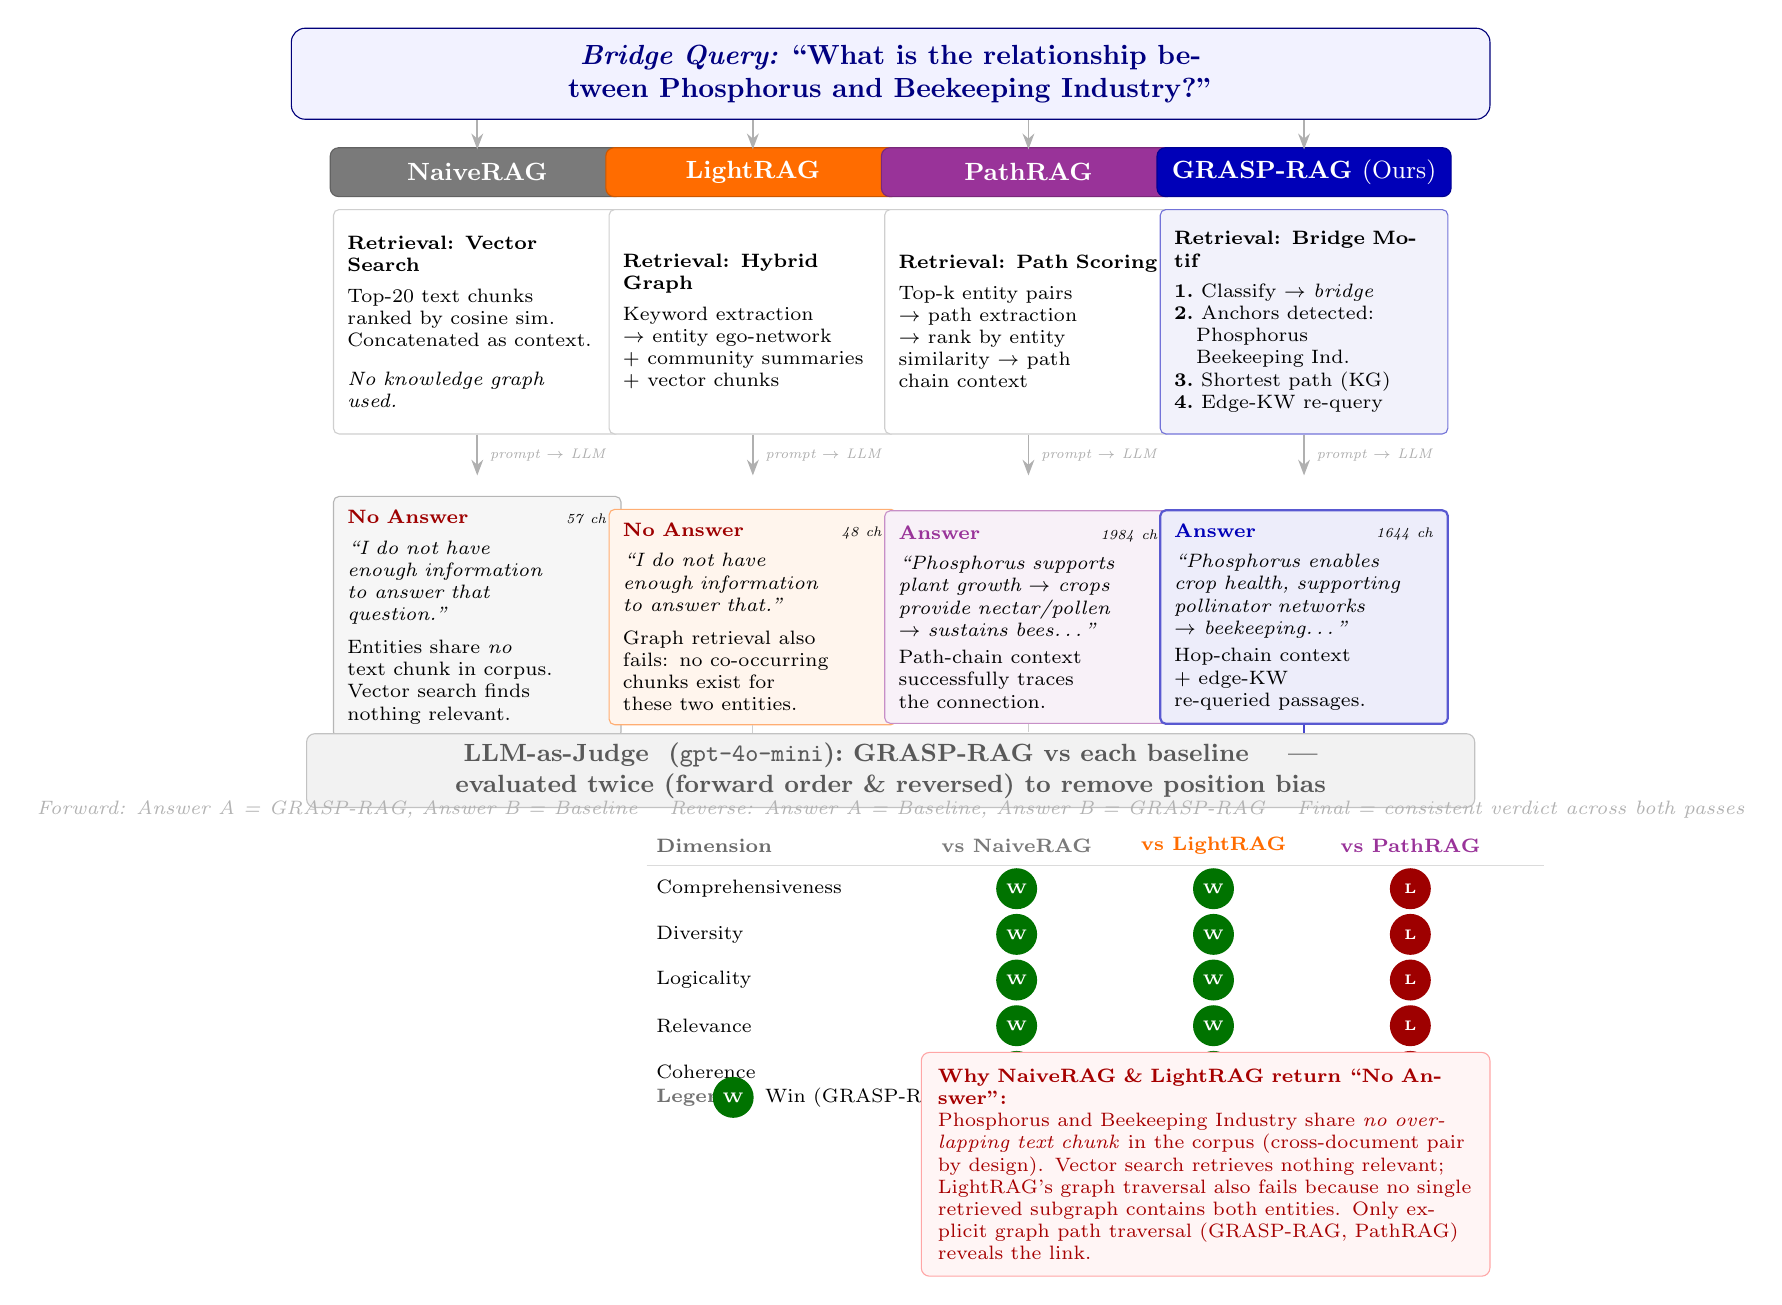
\begin{tikzpicture}[font=\small, >=Stealth]

%% ── Column centres ───────────────────────────────────────────────────────────
\def\xN{-5.25}   % NaiveRAG
\def\xL{-1.75}   % LightRAG
\def\xP{ 1.75}   % PathRAG
\def\xG{ 5.25}   % GRASP-RAG

%% ════════════════════════════════════════════════════════
%%  ROW 0 — Query
%% ════════════════════════════════════════════════════════
\node[draw=blue!48!black, fill=blue!5, rounded corners=5pt,
      text width=14.8cm, minimum height=0.9cm,
      align=center, font=\normalsize\bfseries, text=blue!50!black, inner sep=6pt]
  (Q) at (0,0)
  {\textit{Bridge Query:}\ ``What is the relationship between
   \textbf{Phosphorus} and \textbf{Beekeeping Industry}?''};

%% ════════════════════════════════════════════════════════
%%  ROW 1 — Method headers
%% ════════════════════════════════════════════════════════
\node[MH=cN] (HN) at (\xN,-1.25) {NaiveRAG};
\node[MH=cL] (HL) at (\xL,-1.25) {LightRAG};
\node[MH=cP] (HP) at (\xP,-1.25) {PathRAG};
\node[MH=cG] (HG) at (\xG,-1.25) {\textbf{GRASP-RAG}\ \textnormal{(Ours)}};

\foreach \x in {\xN,\xL,\xP,\xG}
  \draw[Arr] (Q.south -| \x,0) -- (\x,-0.96);

%% ════════════════════════════════════════════════════════
%%  ROW 2 — Retrieval description
%% ════════════════════════════════════════════════════════
\node[RB] (RN) at (\xN,-3.15) {
  \textbf{Retrieval: Vector Search}\\[3pt]
  Top-20 text chunks\\ranked by cosine sim.\\
  Concatenated as context.\\[6pt]
  \textit{No knowledge graph\\used.}
};
\node[RB] (RL) at (\xL,-3.15) {
  \textbf{Retrieval: Hybrid Graph}\\[3pt]
  Keyword extraction\\
  $\to$ entity ego-network\\
  $+$ community summaries\\
  $+$ vector chunks
};
\node[RB] (RP) at (\xP,-3.15) {
  \textbf{Retrieval: Path Scoring}\\[3pt]
  Top-k entity pairs\\
  $\to$ path extraction\\
  $\to$ rank by entity\\
  similarity $\to$ path\\
  chain context
};
\node[RB, draw=cG!55, fill=cG!5] (RG) at (\xG,-3.15) {
  \textbf{Retrieval: Bridge Motif}\\[3pt]
  \textbf{1.}~Classify $\to$ \textit{bridge}\\
  \textbf{2.}~Anchors detected:\\
  \quad Phosphorus\\
  \quad Beekeeping Ind.\\
  \textbf{3.}~Shortest path (KG)\\
  \textbf{4.}~Edge-KW re-query
};

%% ════════════════════════════════════════════════════════
%%  ROW 2.5 — "Prompt → LLM" arrows
%% ════════════════════════════════════════════════════════
\foreach \n in {N,L,P,G}
  \draw[Arr] (R\n.south) -- node[PL]{prompt $\to$ LLM} ++(0,-0.52);

%% ════════════════════════════════════════════════════════
%%  ROW 3 — Answers
%% ════════════════════════════════════════════════════════
\node[AB=cN] (AN) at (\xN,-6.9) {
  \textcolor{cLoss}{\textbf{No Answer}}\hfill\textit{\tiny 57 ch}\\[3pt]
  \textit{``I do not have\\enough information\\to answer that\\question.''}\\[4pt]
  Entities share \emph{no}\\text chunk in corpus.\\Vector search finds\\nothing relevant.
};
\node[AB=cL] (AL) at (\xL,-6.9) {
  \textcolor{cLoss}{\textbf{No Answer}}\hfill\textit{\tiny 48 ch}\\[3pt]
  \textit{``I do not have\\enough information\\to answer that.''}\\[4pt]
  Graph retrieval also\\fails: no co-occurring\\chunks exist for\\these two entities.
};
\node[AB=cP] (AP) at (\xP,-6.9) {
  \textcolor{cP}{\textbf{Answer}}\hfill\textit{\tiny 1984 ch}\\[3pt]
  \textit{``Phosphorus supports\\plant growth $\to$ crops\\provide nectar/pollen\\$\to$ sustains bees\ldots''}\\[2pt]
  Path-chain context\\successfully traces\\the connection.
};
\node[AB=cG, draw=cG!65, line width=0.8pt] (AG) at (\xG,-6.9) {
  \textcolor{cG}{\textbf{Answer}}\hfill\textit{\tiny 1644 ch}\\[3pt]
  \textit{``Phosphorus enables\\crop health, supporting\\pollinator networks\\$\to$ beekeeping\ldots''}\\[2pt]
  Hop-chain context\\$+$ edge-KW\\re-queried passages.
};

%% ════════════════════════════════════════════════════════
%%  ROW 4 — Judge section
%% ════════════════════════════════════════════════════════

%% Arrows answer → judge
\draw[Arr, cG!72, thick]    (AG.south) -- ++(0,-0.52);
\draw[Arr, gray!38, dashed, thin] (AN.south) -- (\xN,-8.55);
\draw[Arr, gray!38, dashed, thin] (AL.south) -- (\xL,-8.55);
\draw[Arr, gray!38, dashed, thin] (AP.south) -- (\xP,-8.55);

%% Judge header
\node[JBar] (JH) at (0,-8.85){
  LLM-as-Judge \ (\texttt{gpt-4o-mini}):\ GRASP-RAG vs each baseline
  \quad---\quad
  evaluated twice (forward order \& reversed) to remove position bias
};

%% Prompt structure note under header
\node[font=\scriptsize\itshape, text=gray!60, align=center]
  at (0,-9.35)
  {Forward: Answer A = GRASP-RAG, Answer B = Baseline \quad
   Reverse: Answer A = Baseline, Answer B = GRASP-RAG \quad
   Final = consistent verdict across both passes};

%% Table column headers
\node[font=\scriptsize\bfseries, text=black!58, anchor=west] at (-3.1,-9.8)  {Dimension};
\node[font=\scriptsize\bfseries, text=cN] at ( 1.6,-9.8) {vs NaiveRAG};
\node[font=\scriptsize\bfseries, text=cL] at ( 4.1,-9.8) {vs LightRAG};
\node[font=\scriptsize\bfseries, text=cP] at ( 6.6,-9.8) {vs PathRAG};

\draw[gray!28, thin] (-3.1,-10.05) -- (8.3,-10.05);

%% Table rows (5 dimensions × 3 baselines)
\foreach \i/\dim in {
  0/Comprehensiveness,
  1/Diversity,
  2/Logicality,
  3/Relevance,
  4/Coherence}{
  \pgfmathsetmacro{\ry}{-10.35 - \i*0.58}
  \node[font=\scriptsize, anchor=west] at (-3.1,\ry) {\dim};
  \node[Vc, fill=cWin]  at (1.6,\ry) {\textbf{W}};   % vs NaiveRAG
  \node[Vc, fill=cWin]  at (4.1,\ry) {\textbf{W}};   % vs LightRAG
  \node[Vc, fill=cLoss] at (6.6,\ry) {\textbf{L}};   % vs PathRAG
}

%% Legend
\node[font=\scriptsize\bfseries, text=black!55, anchor=west] at (-3.1,-13.0) {Legend:};
\node[Vc, fill=cWin]   at (-2.0,-13.0) {\textbf{W}};
\node[font=\scriptsize, anchor=west] at (-1.72,-13.0) {Win (GRASP-RAG better)};
\node[Vc, fill=cLoss]  at ( 1.0,-13.0) {\textbf{L}};
\node[font=\scriptsize, anchor=west] at ( 1.28,-13.0) {Loss (baseline better)};
\node[Vc, fill=gray!55] at ( 4.0,-13.0) {\textbf{T}};
\node[font=\scriptsize, anchor=west] at ( 4.28,-13.0) {Tie};

%% Cross-document annotation
\node[draw=red!35, fill=red!4, rounded corners=3pt,
      text width=6.8cm, font=\scriptsize, inner sep=6pt, align=left,
      text=red!65!black]
  at (4.0,-13.85) {
  \textbf{Why NaiveRAG \& LightRAG return ``No Answer'':}\\
  Phosphorus and Beekeeping Industry share
  \emph{no overlapping text chunk} in the corpus
  (cross-document pair by design).
  Vector search retrieves nothing relevant;
  LightRAG's graph traversal also fails
  because no single retrieved subgraph
  contains both entities.
  Only explicit graph path traversal
  (GRASP-RAG, PathRAG) reveals the link.
};

\end{tikzpicture}
\end{document}
